\chapter{Parameters and Configurations in RSCAD}\label{Appendix_D}

\section{Reactive power control parameters in DVC}

\begin{table}[H]
\centering
\begin{tabular}{|c|c|c|c|}
\hline
\textbf{Parameter} & \textbf{Description}                                      & \textbf{Unit} & \textbf{Value} \\ \hline
$k_{QV}$           & Static gain for slow global reactive power control        & p.u.          & 6.6            \\ \hline
$q_{vsc\_max/min}$ & Maximum/minimum reactive power                            & p.u.          & 0.31           \\ \hline
$k_Q$              & Slow global reactive power control proportional gain      & p.u.          & 0.002          \\ \hline
$T_Q$              & Slow global reactive power control integral time constant & s             & 15             \\ \hline
$k_V$              & Fast local voltage control proportional gain              & p.u.          & 0.2            \\ \hline
$x$                & Converter reactance                                       & p.u.          & 0.1            \\ \hline
$k_P$              & Washout filter proportional gain                          & p.u.          & 0.05           \\ \hline
$T_w$              & Washout filter time constant                              & s             & 0.01           \\ \hline
\end{tabular}
\caption{Parameters of reactive power control loop in DVC}
\label{tab:Reactive_pow_para}
\end{table}

\section{Active power control parameters in DVC}

\begin{table}[H]
\centering
\begin{tabular}{|c|c|c|c|}
\hline
\textbf{Parameter} & \textbf{Description}                                  & \textbf{Unit} & \textbf{Value} \\ \hline
$k_S$              & DC voltage control proportional gain                  & p.u.          & 1              \\ \hline
$T_S$              & DC voltage control integral time constant             & p.u.          & 0.1            \\ \hline
$k_{Rf}$           & Proportional gain for direct frequency control        & p.u.          & 1              \\ \hline
$T_{Rf}$           & First order delay for direct frequency control        & s             & 0.2            \\ \hline
$T_{U_v}$ & \begin{tabular}[c]{@{}c@{}}Washout time constant for the voltage dependent active power\\ reduction\end{tabular} & s    & 60    \\ \hline
$k_{Ufv}$ & Proportional gain for voltage dependent active power reduction                                                   & p.u. & 2     \\ \hline
$T_{Ufv}$ & \begin{tabular}[c]{@{}c@{}}First order delay for the voltage dependent active power\\ reduction\end{tabular}     & s    & 0.005 \\ \hline
$x$                & Converter reactance                                   & p.u.            & 0.1            \\ \hline
$k_Q$              & Washout filter proportional gain                      & p.u.          & 0.05           \\ \hline
$T_w$              & Washout filter time constant                          & s             & 0.01           \\ \hline
$T_a$              & Voltage measurement delay                             & s             & 5              \\ \hline
                   & Deadband for direct frequency control                 & Hz            & 0.2            \\ \hline
                   & Deadband for voltage dependent active power reduction & p.u.          & 0.1            \\ \hline
\end{tabular}
\caption{Parameters of active power control loop in DVC}
\label{tab:Active_pow_para}
\end{table}

\section{V/F control parameters}
\begin{table}[H]
\centering
\begin{tabular}{|c|c|c|}
\hline
\textbf{Parameter}  & \textbf{Unit}
& \textbf{Value} \\ \hline
$k_{p\_vf}$     & p.u. & 0.2 \\ \hline
$k_{i\_vf}$     & p.u. & 30 \\ \hline
\end{tabular}
\caption{Parameters for PI gains in V/F control loop \cite{vrana2013cigre}}
\label{tab:U_F_para}
\end{table}





\section{Cable module configuration}\label{config_cable}
The cable module opens a cable setup popup menu into which the cable parameters are added. The file is then compiled and saved in a ".clo" file format. The cable parameters are referenced through the external file previously created using the cable module. In RSCAD, Pi cable models are derived from Bergeron cable model. Initially, a Bergeron cable model is created with RLC parameters and then the option to make it work as a Pi model is chosen. The ".clo" file must be added first using the 'Dnm1' option, which is obtained by double-clicking on the calculation box (Figure \ref{fig:CableConfig}). The cable constants are of type Bergeron as chosen in the 'cntyp' parameter in Figure \ref{fig:CableConfig}. The 'frcpi' parameter available in the "Options when using Bergeron data" tab, forces the use of Pi section model manually by the user. The selection is made, as shown by the red box in Figure \ref{fig:CabAddit}. The terminal block must be specified as either the sending or receiving end as shown in Figure \ref{fig:Terminal_options} and the cable name provided in the calculation block has to be entered in the terminal blocks as well.\\

\begin{figure}[H]
\centering
\subfloat[Cable configuration]{\label{fig:CableConfig}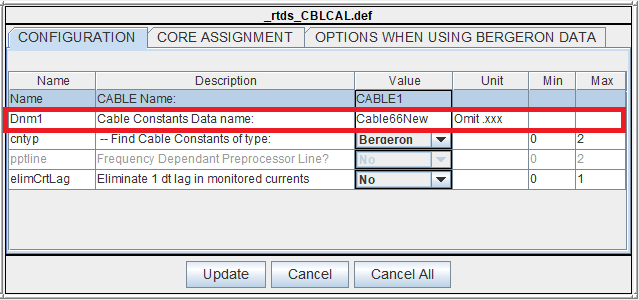
\includegraphics[width=.5\linewidth]{Diagrams/Chapter_3/CableParaBlockInside1.PNG}}\hfill
\subfloat[Additional options]{\label{fig:CabAddit}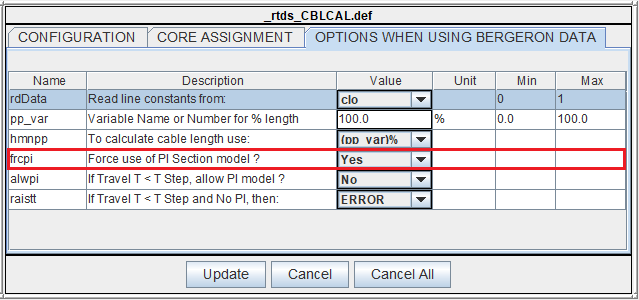
\includegraphics[width=.5\linewidth]{Diagrams/Chapter_3/CableParaBlockInside2_mark.png}}
\caption{Configuration of the calculation block}
\label{fig}
\end{figure}

\begin{figure}[H]
\centering
\begin{subfigure}{0.5\textwidth}
  \centering
  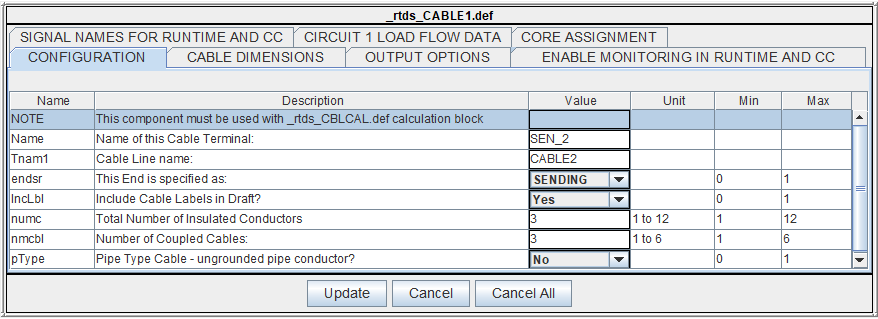
\includegraphics[height = 4cm,width = 8.5cm]{Diagrams/Chapter_3/CableParaBlock_sen_term.PNG}
  \caption{Sending end terminal}
  \label{fig:CableParaBlock_sen_term}
\end{subfigure}%
\begin{subfigure}{0.5\textwidth}
  \centering
  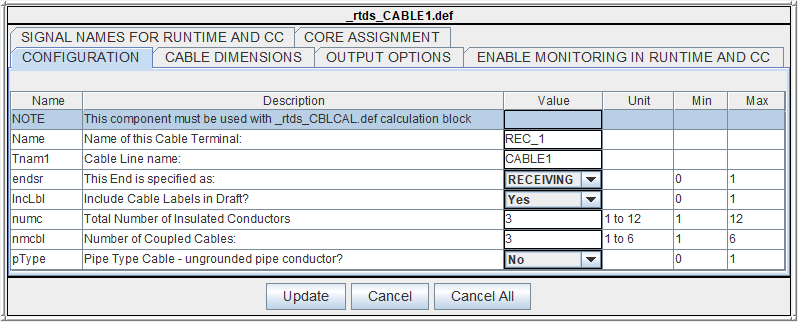
\includegraphics[height = 4cm,width = 8.5cm]{Diagrams/Chapter_3/CableParaBlock_rec_term.PNG}
  \caption{Receiving end terminal}
  \label{fig:CableParaBlock_rec_term}
\end{subfigure}
\caption{Configuration of the terminal blocks}
\label{fig:Terminal_options}
\end{figure}

\section{Core assignment in RSCAD}
\begin{figure}[H]
\begin{subfigure}{.5\textwidth}
  \centering
  % include first image
  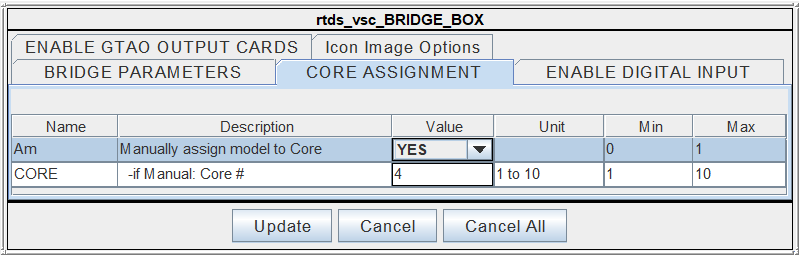
\includegraphics[height = 3cm,width = 8cm]{Diagrams/Chapter_4/Core_assignment_OWF1.PNG}  
  \caption{Core assignment of OWF-1}
  \label{fig:Core_assignment_OWF1}
\end{subfigure}
\begin{subfigure}{.5\textwidth}
  \centering
  % include second image
  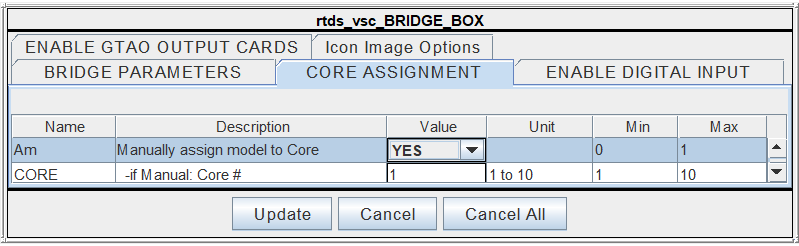
\includegraphics[height = 3cm,width = 8cm]{Diagrams/Chapter_4/Core_assignment_OWF2.PNG}  
  \caption{Core assignment of OWF-2}
  \label{fig:Core_assignment_OWF2}
\end{subfigure}

\newline

\begin{subfigure}{.5\textwidth}
  \centering
  % include third image
  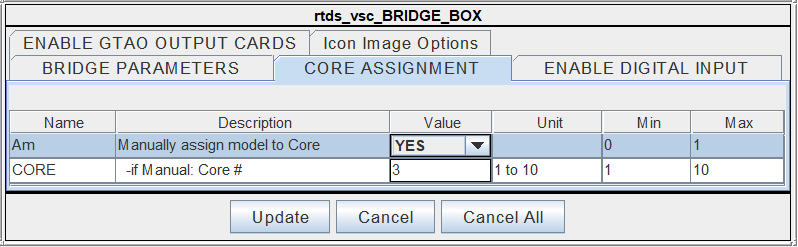
\includegraphics[height = 3cm,width = 8cm]{Diagrams/Chapter_4/Core_assignment_OWF3.PNG}  
  \caption{Core assignment of OWF-3}
  \label{fig:Core_assignment_OWF3}
\end{subfigure}
\begin{subfigure}{.5\textwidth}
  \centering
  % include fourth image
  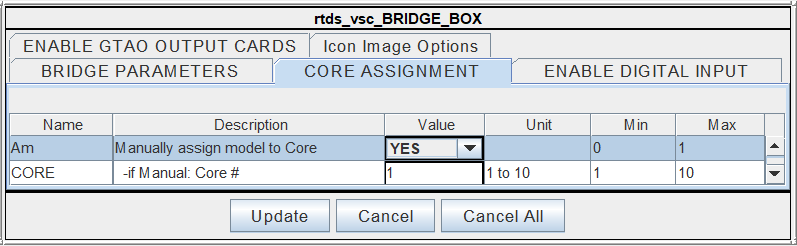
\includegraphics[height = 3cm,width = 8cm]{Diagrams/Chapter_4/Core_assignment_OWF4.PNG}  
  \caption{Core assignment of OWF-4}
  \label{fig:Core_assignment_OWF4}
\end{subfigure}
\caption{Core assignment of the 4 small time step boxes representing 4 OWFs}
\label{fig:Complete_Core_assignment_OWF}
\end{figure}

After assigning the cores for the small time step blocks, the processor assignment for subsystem 2 is as illustrated in Figure \ref{fig:subsystem2_processor}. The 'Core Assignment' tab is available by right-clicking the small time block and choosing "Edit" and then "Parameters" as shown in Figure \ref{fig:Complete_Core_assignment_OWF}. Setting the 'Am' parameter to 'No' for all the small time blocks causes all the available cores to be full and leaving no room for a processor to allocate control signals. Hence these cores should be manually assigned, and proper allocation has to be done.

\begin{figure}[H]
\centering
%\hspace*{-2.2cm}
    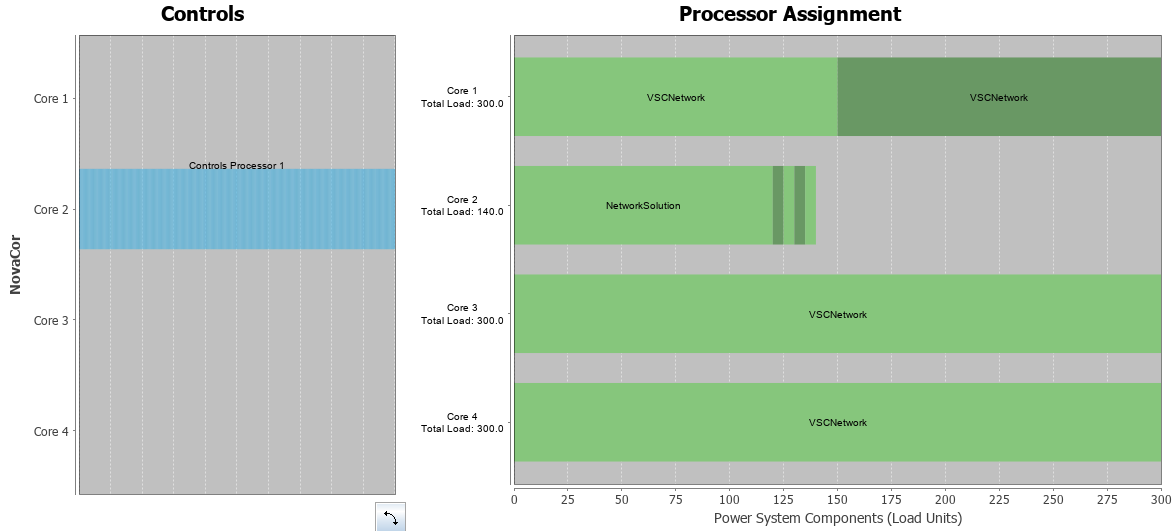
\includegraphics[height = 8cm,width = 17cm]{Diagrams/Chapter_4/subsystem2_processor.PNG}
    \caption{Processor assignment chart for subsystem 2}
    \label{fig:subsystem2_processor}
\end{figure}


\section{Tline module configuration}\label{config_Tline}
The parameters are entered in the Tline popup menu, and the file is compiled and saved in a ".clo" format.

The cable parameters are referenced through the external file previously created using the cable module. %Initially, a Bergeron cable model is created with RLC parameters in the Tline module. 
The ".clo" file must be added first using the 'Dnm1' option, which is obtained by double-clicking on the calculation box (Figure \ref{fig:Tline_calculationbox_RSCAD}). The cable constants are of type Bergeron as chosen in the 'cntyp' parameter in Figure \ref{fig:CableConfig}.

\begin{figure}[H]
  \centering
  % include second image
  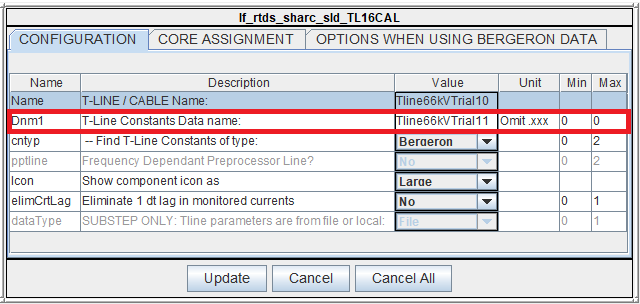
\includegraphics[height = 4cm,width = 9cm]{Diagrams/Chapter_4/TlineParaBlock_side1_mark.png}  
  \caption{Configuring Tline model in RSCAD}
  \label{fig:Tline_config_RSCAD}
\end{figure}

\section{Representation of symmetrical monopole configuration in RSCAD}\label{monopole_rep_RSCAD}
\begin{figure}[H]
\centering
%\hspace*{-1.2cm}
\begin{subfigure}{.5\textwidth}
  \centering
  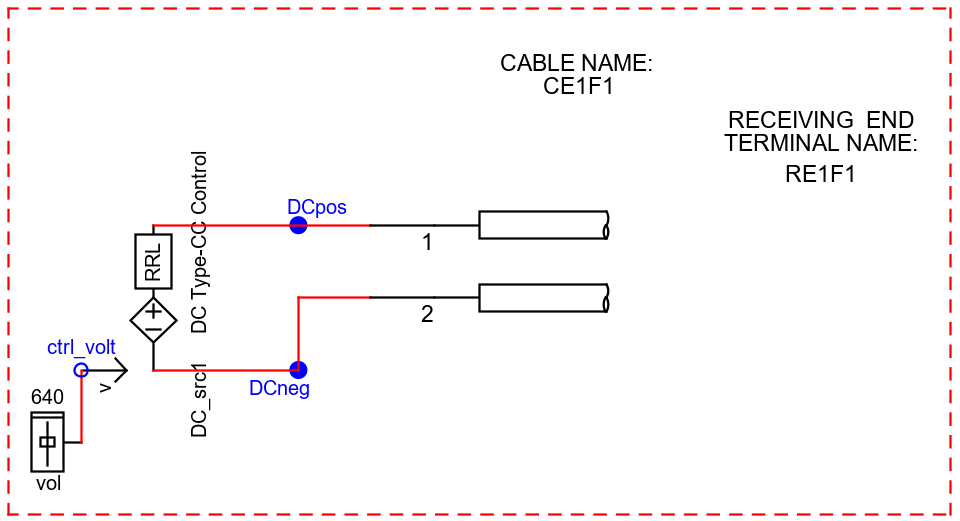
\includegraphics[height=4.5cm,width=8.5cm]{Diagrams/Chapter_4/DC_Source_Cab1.PNG}
  \caption{DC source-1 connected to the receiving end of HVDC cable-1}
  \label{DC_Source_Cab1}
\end{subfigure}%
\begin{subfigure}{.5\textwidth}
  \centering
  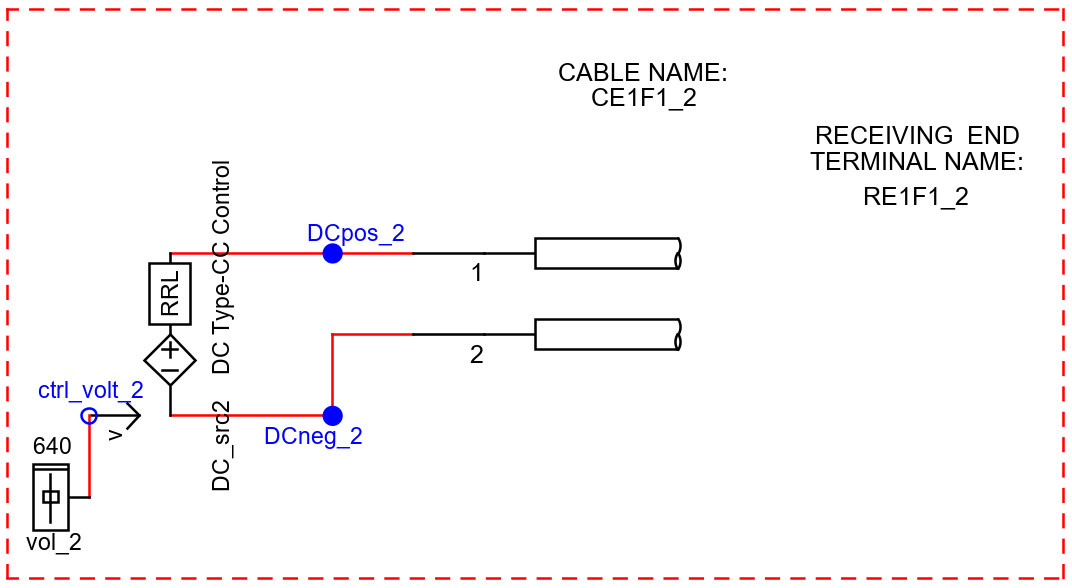
\includegraphics[height=4.5cm,width=8.5cm]{Diagrams/Chapter_4/DC_Source_Cab2.PNG}
  \caption{DC source-2 connected to the receiving end of HVDC cable-2}
  \label{DC_Source_Cab2}
\end{subfigure}
\caption{Onshore converter stations representation using DC sources in RSCAD}
\label{fig:DC_source_cab}
\end{figure}


%The outer control loop model available in \cite{vrana2013cigre} is suitable for 145 kV \gls{HVAC} network. Hence, for the 66 kV \gls{HVAC} network developed for this work, the outer loop is simplified and the reference values ($i_{d\_ref\_2}$ and $i_{q\_ref\_2}$) for the inner control loop is directly defined by the user.

